\section{Introduction}
Convolutional neural networks (CNNs) for object detection are being  heavily adopted in the perception task of autonomous systems.
%
Despite the power of CNNs at being able to learn complicated patterns from complex environments and producing highly non linear decision boundaries, yet they are still prone to outputting miss-classifications~\cite{Ghobrial2022}. 
%
Affected by the black box nature of CNNs in computing predictions, it makes validation of outputted predictions during operation challenging.
% the task of validation of the classifier's outputs during operation infeasible. 
%
This may hinder the deployment of autonomous systems employing such CNNs.
%
We propose that confidence can be gained to deploy such systems if the system continuously provides certain levels of trustworthiness in their predictions during operation.
%
In this paper we introduce the \textit{trustworthiness score (TS)}, a metric that attempts to provide a scalar quantification of trustworthiness in CNN predictions. 
%
This is achieved by monitoring and checking for overlaps of \textit{features specifications} with predictions. 
%
The term features specifications is used here to refer to unique distinctive properties that make up a classification class.
%  
%
The TS metric can serve as an online monitoring tool to improve the evaluation of CNNs trustworthy predictions during operation. We also explore if a modification of the TS metric can be used to calculate a suspiciousness score (SS), which may help in the detection of suspicious frames where False Negatives exist.
% nd assist with miss-classifications detection. 
%
% This may serve as an assistant to the ground truth monitor (human) in monitoring, or substitute the ground truth where it is infeasible to have a human ground truth monitor.
%
In the rest of this paper we discuss related works in section~\ref{sec:related_work}. In section~\ref{sec:method} we introduce our method.
%
Section~\ref{sec:experiment} and ~\ref{sec:results}, show cases our approach and discusses results using the detection of persons as a case study.
%
We conclude in section~\ref{sec:conclusions}.

% The method of adapting to PoL tasks complements the verification and validation work on ASs to achieve deployment. This follows a two-stage approach presented by Koopman et.al. \cite{Koopman2020}, which stipulates that, given an AS passes some minimum safety validation case, the system is deployed and is improved during operation to increase its reliability over time. Thus, the system is allowed to adapt to dynamically changing operational environments which may often vary from the expected operational environment at deployment time.



% ====================

% Include discussion of anomaly detectors in the literature and how it is not sufficient for safety critical systems as the ground truth is reliant on the model of what is "normal"? This goes takes us back to the issue of transparency and other limitations of using Neural networks in safety critical applications. \cite{paper from Seth Bullock}

% Bare this paper in mind as a way of defining a threshold for to gain confidence in the features specifications defined or expressed using other DNNs (e.g. detecting eye noise etc.) to monitor the main DNN (e.g. which detects a whole human)~\cite{Hendrycks2017}.


% Point that was mentioned by Andrew Banks from LDRA or MISRA C: Toyota got fined several millions for quality failure because  their code was too complicated. No one found a bug and it was not possible to verify the code because it was too complicated. Similarly ML is like a black hole, you feed in data and somehow it gives you a result. To avoid such failures of the system when the system is too complicated, we need to sanitise our inputs to the system, thus avoid garbage in garbage out. However you can also have a completely fine and valid input but the output could be wrong (still garbage out) so we also need to validate the decision making. This is where explainability becomes crucial. Our paper aims at validating these outputs by creating features specifications for the classification of objects. Thus the output of a system can be validated against these features specification by calculating a confidence between what features should be used in classification decision vs what the system  the intersections between the causality explanations using a metric that evaluates the confidence in classification by. 

% ===============================

% Trust can be defined subjectively based on the field of usage. The definition that aligns the closest with the focus of this paper out of several that exist is: ``\textit{trust is a belief level of an object to other objects based on direct observations (and previous observations)}''~\cite{Najib2019}.

% Trust in Classification Score (TS), is therefore a score that dictates whether a classifier's output for a given frame or image should be relied upon or not . 



\section{Related Work}\label{sec:related_work}
%
% using explainability in machine learning and features specficiations  explanations and reasoning similar to humans reasoning of trust.Thus can be used in   and can be used to provide accountability \textit{Trust in Classification Score}
%
We discuss briefly relevant parts of trust in humans vs trustworthiness, overview existing works relating to trust calculations in machine learning (ML), discuss why existing methods are insufficient as trustworthiness metrics, contrast our proposed approach against the notion of \textit{uncertainty quantification} in ML and lastly review explainability techniques relevant to our proposed methodology. 
%
% \textcolor{red}{
%, often represented as a probability that a model will make the correct decision.}



\subsection{Trust and Trustworthiness}\label{trustVStrustowrthiness}
\textit{Trust} is a term that is conceptually used to express a trustor's (someone) subjective estimate of the probability that the trustee (someone or something) will display the trustor's preferred behaviour~\cite{Bauer2013}.
%
Therefore trust as interpreted by humans is a measure of subjective confidence and may vary and evolve dependant on an individual's personal set of skills and experiences~\cite{Hommel2015, Mitkidis2017,Najib2019}. 
% This aligns with the hypothesis that trust in humans is largely reliant on the degree of interpersonal similarities, which may .  
% Trust in humans is usually based on interpersonal similarity as discussed in \cite{Mitkidis2017}.
%
\textit{Trustworthiness} on the other hand, whilst also being a measure of confidence, is evaluated based on the trustee demonstrating a certain set of established characteristics that prove they are doing the \textit{correct} behaviour based on some ground truth reference~\cite{Bauer2013, Bournival2022}.
%
These demonstrable characteristics vary depending on the application and on whether the trustee being a human or a machine~\cite{Wing2021}.
%
Trust and trustworthiness tends to be used interchangeable in some ML literature~\cite{DeBie2021,Jiang2018}.
%
Following definitions discussed above we distinguish between trust and trustworthiness: trust being a subjective measure of confidence based on experiences and hence is best for usage between human to human interactions, while trustworthiness is based on demonstrating that the \textit{correct} behaviour (grounded by a set of characteristics) is pursued and thus is more suitable for runtime evaluation of ML predictions. 
%
Access to ground truth or a reference point is required to check for the \textit{correctness} likelihood of a prediction~\cite{Barr2015}, making the demonstration of a system's trustworthiness troublesome during runtime.

Jiang et.al.~\cite{Jiang2018} introduced the \textit{trust score}, which considers a prediction as trustworthy if the operating classifier's prediction aligns with the nearest-neighbor classifier's output based on the training data. Here the nearest-neighbor classifier based on the training data is the reference point. However, Jiang's trustworthiness calculation lack's transparency and explainability.
%
De Bie et.al.~\cite{DeBie2021} tried to overcome the explainability limitation with RETRO-VIZ. This method takes a very similar approach as Jiang et.al.\cite{Jiang2018} in calculating the trustworthiness using the trust score, but replaces the ground truth output of the nearest neighbour classifier with the output from a \textit{reference set}. The reference set is extracted from the training data using similarity measures~\cite{Hond2020} (e.g. euclidean distance) to select data points similar to the input data point. 
%
Additionally they try to improve upon Jiang et.al.'s approach by producing a visualisation that help understand the reasons for the estimated trustworthiness based on features from the reference set. This aims at providing a justification to why a prediction was assigned a certain trust score. However it does not ensure the trustworthiness is calculated based on the existence of certain features or characteristics that are demonstrable in the prediction.%, and thus should make up a trustworthy prediction. 

Both approaches by Jiang and De Bie fit better under \textit{trust} %(subjective)
calculations, which we differentiate from trustworthiness as outlined above:  trustworthiness should be calculated based on certain characteristics found in a prediction rather than calculating the trustworthiness first based on hidden features then trying to explain it to find which features credited trustworthiness. Additionally their approaches benefit from alleviating the engineering effort needed to identify which features should matter in calculating the trustworthiness score, but as a result it may lead to misleading and unworthy trustworthiness scores if used in operation.
% by finding similarity in scores between these hidden features and other  characteristics that were used in calcuating the trustworhtiness.
%
%If the classifer's output  Thus determine whether the output of the operating classifier $h$ would be trustworthy or not. 
%
We overcome this limitation in this paper by taking an interrogative approach in assessing the operating classifier's predictions based on established characteristics/features that are chosen and approved should be monitored during operation. Based on these features being evident and demonstrable a trustworthiness score is assigned to the prediction.
%
% should be demonstrable in a prediction and consequently based on the evidence found we assign a trustworthiness score. 
% Due to the design nature of our approach it is transparent and thus interpretable even by non-domain experts.
% The approach we introduce in this paper for calculating the trustworthiness takes an interogative approach at calculate the trustworhtiness of a classifer's predction. Instead of  
%
% i) The methods may do not provide explanations
% Just as Both of these methods do not provide explanations to why these methods are not trustworthy, and the trustwothiness expalnations  
% This method of evaluating the similarity between input data and training data has also been used to verify or estimate the uncertainty of a classifier's output~\cite{Hond2020}.
% \cite{Najib2019}

Paudel et.al. introduced ConsensusNet, which is targeted at learning correlations between predictions assigned to different cells in an image by a classifier.% (e.g.YOLO~\cite{Redmon2018}). 
%
These correlations are hypothesised to hold for training data and operational input data. If these correlations do not hold, then the output of the classifier is considered to be a miss-classification~\cite{Paudel2021}. 
%
The method we introduce
% for measuring the trustworthiness of classifications 
does not use Paudel et.al.'s method of assessing correlation between grid cells
%of an image
, but we do share the underlying idea of different features that make up a label class should be monitored during operation to identify miss-classifications.

\subsection{Uncertainty in Machine Learning}
\textit{Uncertainty quantification} in ML is used to represent probabilistically the level of unknown information in a prediction, thus enabling users when to trust a model's prediction~\cite{ghahramani2015probabilistic}\cite{tran2022plex}.
%
One popular way for computing uncertainty is by utilising Bayesian inference in the model's architecture to output a distribution of uncertainties over outputs~\cite{gal2016dropout}\cite{ABDAR2021}. 
%
A drawback of that, is the need to do changes in the architecture of the neural network e.g.~\cite{Kraus2019}.
%
The trust score discussed earlier introduced by Jiang et.al. ~\cite{Jiang2018} overcomes the need to change the network structure and outputs only a score rather than a distribution.
%
Our \textit{trustworthiness score} excels beyond the aforementioned trust score in the transparency aspect, which may be very advantageous especially in human-computing interaction applications. 
%
Furthermore, classification with a reject option, where the model is enabled to abstain from a making a prediction is very relatable to our method~\cite{hendrickx2021machine}. 
%
An advantage of our method, is that the model is treated as a black box, whilst often classifiers with a reject option rely on learning a classification and a rejection function simultaneously. 


\subsection{Interpretability in Machine Learning}
In the context of ML, \textit{interpretability} has been very nicely defined as the ``ability to explain or to present in understandable terms to a human''~\cite{Doshi-Velez2017}. 
%
In turn, interpretability allows users to trust or distrust classifiers~\cite{Rudin2022}. 
%
Interpretability seems to be a requirement for generating trust in classifiers' predictions~\cite{Ribeiro2016, Lipton2018}, however in ~\cite{Lipton2018} it has been also argued that trust does not necessarily rely on interpretability. This latter argument can be backed up by the trust score introduced by Jiang et.al.~\cite{Jiang2018}, which does not rely on interpretability. 
%
However, motivated by our earlier discussion between trust and trustworthiness in section~\ref{trustVStrustowrthiness}, trustworthiness requires demonstrability therefore having interpretable \textit{explanations} becomes a requirement to generate trustworthiness in predictions.
%
% Hence, explanations generation of predictions forms a corner stone in calculating our trustworthiness score. 
%
% There are several methods for generating interpretable explanations for object classifiers in the literature e.g. GradCam~\cite{Selvaraju2020}, LIME~\cite{Ribeiro2016}, SHAP~\cite{Lundberg2017}, Extremal~\cite{Fong2019}, DeepCover~\cite{Sun2020}. All of these methods are developed for generating explanations for classifiers that output only a label (i.e. without a bounding box localising the classification). 
% %
% Our method works for both types of classifiers, ones that output only a label and ones that output a label and a bounding box. Where the classifier only outputs a label, an explanation technique is required to allow for the calculation of the trustworthiness in classification score.



\section{Method} \label{sec:method}
% Validating a software against its set of specifications provides developers with the trustworthiness needed for deployment. Motivated by this idea, we developed our trustworthiness score (TS) metric. 
An overview of the process used to calculate the trustworthiness score (TS) in predictions and the suspiciousness score in a frame is shown by 
Figure~\ref{fig:method_overview}. 
%
We use the term \textit{main classifier} to refer to the CNN responsible for object recognition. 
%
The input image is fed into the main classifier to obtain two sets of predictions. The first set of predictions $\{N_{i,1},..., N_{i,Y_i}\}$ are predictions with model confidence ($MC$) $\geq$ to the set model confidence threshold ($MC_T$). The second set of predictions $\{M_{i,1},..., M_{i,J_i}\}$ is for $MC < MC_T$. Where $Y_i$ and $J_i$ are the total number of predictions detected in image $x_i$ for $MC \geq MC_T$ and $MC<MC_T$ respectively.

Dependent on the type of object recognition the main classifier is designed to undertake, the explanation generation method may differ.
%
% an explanation might or might not need to be generated. If the output of the main classifier is just a label of the object in the image then an explanation needs to be generated, to find which pixels resulted in the classifier's prediction.
% %
% On the other hand if the main classifier outputs a label and a bounding box of the object in the image, then one does not need to generate an explanation, as the bounding box encapsulates the pixels resulted in the output i.e. $N(x_i)\equiv E(x_i)$. 
%
Simultaneously the input image is scanned for features that fit the defined features specifications. Pixels of detected features specifications that overlap with explanation pixels are used in calculating the TS.
%
We discuss below the different parts of our method for calculating TS and we show how following a similar concept of the TS, a suspiciousness score for the image can be calculated using $\{M_{i,1},..., M_{i,J_i}\}$.
\begin{figure*}%[h]
\centering
% \resizebox{!}{100}{
    \begin{tikzpicture}[node distance=3.5cm]
   
    \node (classifier) [process, minimum width=1.5cm, minimum height=1.5cm, text width=1.5cm, text height=0cm, text depth = 0 cm, yshift=0cm, xshift=1cm] {Main Classifier};

    % \node[text width=3cm] at ([xshift=0mm,yshift=-7mm]classifier.east) 
    % {\tiny $MC \geq MC_{T}$};

    % \node[text width=3cm] at ([xshift=0mm,yshift=5mm]classifier.east) 
    % {\tiny $MC < MC_{T}$};

    \node (ss_calculation) [process, right of=classifier, minimum width=2cm, minimum height=1cm, text width=2.5cm, text height=0cm, text depth = 0 cm, yshift=0.5cm, xshift=1cm] {SS Calculation};
    
    
    \node (explanations_generator) [process,  right of=classifier, minimum width=1.5cm, minimum height=1.5cm, text width=2.5cm, text height=0cm, text depth = 0 cm, yshift=-1cm, xshift=1cm, align=center] {Explanations Generator};
    
    \node (features) [process,  below of=classifier, minimum width=1.5cm, minimum height=1.5cm, text width=2cm, text height=0cm, text depth = 0.5 cm, yshift=0.5cm, xshift=-1.7cm, align=center] {Features Specifications Monitor};
    
    \node (tcs_calculation) [process,  below of=explanations_generator, minimum width=2cm, minimum height=1cm, text width=2.5cm, text height=0cm, text depth = 0 cm, yshift=1.5cm, xshift=0cm, align=center] {TS Calculation};
    
     
      \draw[arrow] (-2,0) -- node[anchor=south] {Image $x_{i}$} (classifier);
      
    %   \draw (-1,0) -| node[anchor=south] {} (-1,-2.5);
      
    %   \draw[arrow] (-1,-2.5) -- node[anchor=south] {} (features);
    
    \draw[arrow] (-1,0) -| node[anchor=south] {} (features);
      
      \draw[arrow] ([yshift=-5mm]classifier.east) -- node[anchor=south] {$\{N_{i,1},..., N_{i,Y_i}\}$} ([yshift=5mm]explanations_generator.west);

      \draw[arrow] ([yshift=5mm]classifier.east) -- node[anchor=south] {$\{M_{i,1},..., M_{i,J_i}\}$} ([yshift=0mm]ss_calculation.west);
      
      \draw[arrow] (explanations_generator) -- node[anchor=west] {$\{E_{i,1},..., E_{i,Y_i}\}$} (tcs_calculation);
      
      \draw[arrow] (features) -- node[anchor=south] {$\{F_{i,1},..., F_{i,Z_i}\}$} (tcs_calculation);
      
      \draw[arrow] (tcs_calculation) -- node[anchor=south] {$\{TS_{i,1},..., TS_{i,Y_i}\}$} (10,-3);

      \draw[arrow] (ss_calculation) -- node[anchor=south] {$SS_{i}$} (8,0.5);
       
    \end{tikzpicture}
    % }
\caption{Method Overview}
\label{fig:method_overview}
\end{figure*}

% \todo[inline]{Edit method to add, TS threshold, MC threshold, how TS can be used for suspiciousness in frames}

\subsection{Generating Explanations}
The explanations generator in Figure~\ref{fig:method_overview}
aims at identifying which pixels in image $x_i$ caused the main classifier to output its predictions. Once these pixels are identified an explanation is output where all pixels in image $x_i$ are blacked out (i.e. set to zero) other than the important pixels which resulted in the main classifier prediction. Therefore if the main classifier outputs predictions $\{N_{i,1},..., N_{i,Y_i}\}$ the explanations generator should output a set of explanations $\{E_{i,1},..., E_{i,Y_i}\}$ corresponding to each prediction.  

We distinguish between two types of classifiers targeted at different types of object recognition: 1) object classification, where the object classifier only outputs a label of the most probable item in the displayed image. 2) object detection, where the classifier outputs labels and bounding boxes showing the different objects in the image.
%
For the former, different techniques for generating interpretable explanations for object classification can be used and are available in the literature e.g. GradCam~\cite{Selvaraju2020}, LIME~\cite{Ribeiro2016}, SHAP~\cite{Lundberg2017}, Extremal~\cite{Fong2019}, DeepCover~\cite{Sun2020}. 
%
All of these methods are developed for generating explanations for classifiers that output only a label.% (i.e. without a bounding box localising the classified object). 
%
For the latter type of object recognition, the pixels within the bounding box can be considered as the explanation, e.g.\ $N_{i,1}\equiv E_{i,1}$.
%
% sufficient to represent an explanation, as the bounding box encapsulates the pixels resulted in the output prediction i.e. $N(x_i)\equiv E(x_i)$.
%
Throughout the paper we focus our method on object detection, however, the method can be used in the context of object classification too. 
 

% Inspired by DeepCover~\cite{Sun2020}, Figure~\ref{fig:explanation_generator} shows a flow diagram of how an explanation generator works for the case where the object classifier is of the type that only outputs a label without bounding boxes. For object classifiers that output a label along with a bounding box this step(section) is ignored.
% %
% The image or frame $x_{i,0}$ ($i$ is an image identification number) is inputted in the mutations generator to output a set of $m$ number of mutants $\{x_{i,1}, ... x_{i,j}, .... x_{i,M}\}$ ($j$ is the mutant identification number).
% %
% The mutations generator creates mutants by applying different masking functions to the image whereby only a subset of the pixels in $x_{i,0}$ would be revealed and the rest blacked out.
% %
% The set of generated mutants are evaluated on the main object classifier $N$. A function $A(x_{i,j})$ keeps track of which mutants result in the same output prediction as $y = N(x_{i,0})$ of the original image.

% The image $x_{i,0}$ consists of $m$ pixels $\{ p_1, ... p_k, ... p_m\}$. For each pixel $p_k$ of $x_{i,0}$ the vector $[a_{k,t}, a_{k,f}]^T$ is computed, where $a_{k,t}$ is the number of mutants predicted as $y$ in which $p_k$ is not masked and $a_{k,f}$ is the number of mutants not predicted as $y$ in which $p_k$ is not masked.
% %
% Once the vector $[a_{k,t}, a_{k,f}]$ is calculated for all pixels, they are subtracted from each other using equation~\ref{ranking_equation} to rank the importance of each pixel $p_{k,\text{rank}}$.
% %
% \begin{equation}
% \label{ranking_equation}
% p_{k,rank}=a_{k,t} - a_{k,f}
% \end{equation}
% %
% Pixels ranked from high to low are added to the explanation image $E(x_{i,0})$ gradually until the prediction of the explained image outputs the same prediction (label) as $y$ i.e. $N(E(x_{i,0}))== y$, with confidence in prediction close to the confidence of prediction $y$. The threshold of how close the confidence in label $y$ and $N(E(x_{i,0}))$ is left to the user to determine. 
% % However in our experimentation a threshold of 0.5\% was sufficient to generate explanations with enough fidelity. 
% Where the threshold is set very high, the explanations generated may not be reliable
% % In cases where the threshold is set to be too high, the explanations generated not reliable 
% as the pixels used in the explanation may not be sufficient to provide reasoning of why the classifier allocated its confidence in its prediction i.e. the explanations may lack fidelity to compare features specifications against and use in calculating the TCS.


% \input{GenerateExplanation_v1}
% \input{GenerateExplanation_v2.tex}


\subsection{Features Specifications}
% \todo[inline]{Discuss with Dhaminda for suggestions}
% The motivation
% Motivated by software engineering practices of validating a software against its set of specifications provides developers with the trustworthiness for deployment, we developed our method 

% that a software is fulfills gives use confidence t to full fill, we proposed this method of monitoring distinctive features that make up a class the decision making of the classifier against a set of estbilshed 

% This interrogative way that humans use to justify verify their classifications ()

% What are they?
A \textit{specification} generally ``\textit{is a detailed formulation in document form, which provides a definitive description of a system for the purpose of developing or validating the system}"~\cite{ISO24765}\cite{Dhaminda2022a}. 
%
When defining specifications for features (or features specifications) we aim at unique distinctive properties that make up a classification class. In the rest of this section we discuss how to identify these distinctive features, how to define these features as specifications, and how features specifications can be utilised by machines for monitoring.  

\subsubsection{Identifying Distinctive Features}
 
\begin{itemize}
    \item 
    % \textbf{
    \underline{Method 1, Human logic:} 
    Human labeled data are usually the ground truth used to validate against when it comes to classification. Inspired by that, this approach relies on humans providing a list of distinctive features that has been used in making their personal assessment when labeling data. 
    % In some classification tasks this is very straight forward, e.g. for classifying a person in an image, the distinctive features of person can be the facial landmarks of a human~\cite{Kazemi2014}.
    %
    % \underline{Step1:} 
    \textit{Step~1:} Determine the different classes that the CNN is meant to classify. 
    %
    % \underline{Step2:} 
    \textit{Step~2:} List the distinctive features of each class by analysing through the available dataset. 
    %
    % \underline{Step3}: 
    \textit{Step~3:} Compare between the different distinctive features that were identified for each class and ensure there are no shared distinctive features between classes. In the case where there are shared features, one may want to reflect that in the weighing contribution from that feature in the TCS evaluation.
    %Identify any shared distinctive features between the different classes. %These shared distinctive features will affect the trustworthiness calculation of which class was detected.   
    
% Provides better ground for justification when solving accountability related issues.
% \begin{itemize}
    \item \underline{Method 2, Explainability analysis:} Explainability analysis is targeted at classification tasks where identifying distinctive features to be used as specifications is not intuitive, especially when slight variations in these features can be critical for the classification output~\cite{Antoran2020} e.g. distinctive features of hand written digits.
    %
    The concept utilises powerful explainability techniques readily available in the literature such as LIME~\cite{Ribeiro2016}, SHAP~\cite{Lundberg2017}, CLUE~\cite{Antoran2020} etc., whereby 
    %
    % \underline{
    \textit{Step~1:} the CNN is trained on the data representing the operational environment (training data), 
    %
    % \underline{
    \textit{Step~2:} the training data is fed into the trained model and an explanation is generated for the different data points, 
    %
    % \underline{
    \textit{Step~3:} an analysis is conducted on the generated explanations to identify which features used as common explanations between data points should be regarded as distinctive.
    %
    % These  identified as distinctive features (might want to draw three boxes each showing one of these steps).

    % Defining features Specifications using explanation methods to extract features that are of importance and plays a main role in the classification of an object, this may be of particular interest in applications where defining features specifications is not obvious~\cite{Antoran2020}.


    % \item \textbf{Method 3: Attention Mechanisms features extraction.}
    % Attention mechanisms~\cite{Vaswani2017}\cite{Woo2018} can be used to extract features that play an important role in classification~\cite{Chen2020}. Taking similar steps to the explainability analysis, distinctive features can be derived from attention mechanisms instead of using explainability generation techniques.      
\end{itemize}

\subsubsection{Defining Features as Specifications}
% \todo[inline]{Revise this section}
The different visual features that collectively make up an object in real life, may be challenging to express rigorously using text specifications solely. Therefore, in defining a feature specification, we comprise the specification of two parts: 1) a specification-text and 2) and a specification-visual. 
%
The goal of the specification-text is to describe in natural language what subpart of the object is distinctive and requires monitoring. The specification-visual aids with understanding the extent of the specification-text. 
%
For example, a specification text for monitoring a human palm can be written very simply as ``A person shall have a hand ". This may be interpreted as only the palm of a human, the palm plus the forearm or the whole arm. The specification-visual goal here is to help minimise scope for misinterpretation. 
%
The specification-visual can be a number of example images to represent the feature. This can also be extended to creating a dataset, following assurance of machine learning for use in autonomous systems (AMLAS) guidelines \cite{hawkins2021guidance} to build a dataset representing the specification-visual.
\subsubsection{Describing Features Specifications in Machine Interpretable form}

Once unique features specifications are identified, they need to be expressed in a form that allows machines to  monitor them.
\begin{itemize}
\item \underline{Method 1, Geometrical analysis:} For some features specifications operating in limited environments one could employ image processing to detect these features using geometrical analysis. 
%
Whilst geometrical analysis may be fast and avoids the need to gather data for training, they may result in increased levels of false positives and significant changes in the image processing method used when changing operational environments e.g \cite{Lucian2018}. 

\item \underline{Method 2, Deep Learning:} Many of the features that make up a classification in many operational environments are complex, and hence are difficult to represent using geometrical analysis.
%
Alternatively, one can utilise other CNN models to learn complex features specifications e.g. \cite{Kazemi2014}\cite{Fahn2017}. 

\end{itemize}

\subsection{Trustworthiness Score (TS)}
The trustworthiness score for a given prediction $N_{i,y}$ is calculated using equation~\ref{eq:TS}, where $y\in\{1,..,Y_i\}$. 
%
$R_{i,y,z}$ represents the intersection area between detected feature $F_{i,z}$ and explanation $E_{i,y}$ for prediction $N_{i,y}$. 

\begin{equation}
\label{eq:TS}
    TS_{i,y} = \sideset{}{}\sum_{z=1}^{Z_i} \beta_z \cdot a_{y,z} \cdot R_{i,y,z}%\frac{\sideset{}{}\sum_{z=1}^{Z_i} \beta_z \cdot a_z \cdot R_{i,z}}{Z_i} 
\end{equation}



A trustworthy prediction is shown by the prediction having overlapping features specifications that make the trustworthiness score surpass the set \textit{trustworthiness score threshold}. 
% having  the detected features specifications overlapping with the prediction. 
%
A prediction and a feature count as overlapping if $R_{i,y,z} \geq R_{lim}$. We use $a_{y,z}$ as a boolean switch to indicate if this condition is satisfied or not. $\beta_z$ is included in our equation to act as a hyperparameter for weighing the contribution from different types of detected features specifications.

Determining $R_{lim}$ may depend on the application and type of features specification being monitored. Formalising a method for determining $R_{lim}$ can be scope for future work. However, in our experimentation we have set $R_{lim}$ to $70\%$, as through visual assessment of the outputted bounding boxes (see Figure~\ref{summary_pics}) we deem this to be sufficient to confirm that an overlap exists.    

% % then this provides proof that this feature was used in the main classifier's prediction and the classification is trustworthy against the features specifications.
% %
%  % {$\{F_{i,1},..., F_{i,Z_i}\}$}
% The percentage of pixels $R_{i,z}$ for feature $F_z$ that are not masked in explanation $E(x_{i})$, is given by equation~\ref{percentage_pixels}, where $P$ is a function that calculates the number of non masked pixels in any given set of pixels.
% %
% \begin{equation}
%     \label{percentage_pixels}
%     R_{i,z} = 100 \times \frac{P(F_z \cap E(x_i))}{P(F_z)}
% \end{equation}

% Using $R_{i,z}$ the trustworthiness in classification score is computed using equation~\ref{eq:TCS}, where $z\in\{1,..,Z_i\}$ and $Z_i$ is the total number of features specifications detected in image $x_i$. 
%
% $a_z$ $\in \{1,0\}$ is used to flag whether the detected feature $F_z$ was used in the classifier's prediction, where $a_z = 1$ for $R_{i,z}>=R_{lim}$, otherwise $a_z =  0$.  
% %
% We factor in $\beta_z$ in our equation to weigh the contribution from each feature specification $F_z$ in case the features specified are not all of equal importance. 
% Algorithm~\ref{alg:algorithm} shows an implementation for the TCS calculation.



\subsection{Suspiciousness Score}
We speculate that the trustworthiness score can be modified to detect the suspiciousness in a frame. A frame is referred to as being suspicious if it contains false negatives from the predictions made by the main classifier. 
%
% The baseline used here again relies on the model confidence. For a frame to be suspicious based on model confidence means that the main classifier outputted predictions below the selected main classifier's accuracy. 
%
We modify the TS metric to yield the suspiciousness score (SS) shown by equation~\ref{eq:SS}. 
%
In this case the SS loops over predictions $\{M_{i,1},..., M_{i,J_i}\}$ and sums up the area $R_{i,j}$ of the bounding box for each prediction $M_{i,j}$, where $j\in\{1,..,J_i\}$. 
% below the $MC_threshold$ 
%
% having a low model confidence and sum up their pixels. This can be referred to as the suspiciousness score (SS) and can be expressed using equation-- where...
If SS surpasses some selected \textit{suspiciousness score threshold} then the frame is suspicious. 
\begin{equation}
    SS_i = \sideset{}{}\sum_{j=1}^{J_i} R_{i,j}
    \label{eq:SS}
\end{equation}

% where $j\in\{1,..,J_i\}$ and $J_i$ is the total number of predictions detected in image $x_i$ with model confidence below the selected main classifier's accuracy.

% where $y\in\{1,..,Y_i\}$ and $Y_i$ is the total number of predictions detected in image $x_i$ with model confidence above or equal to the selected main classifier's accuracy.

% $R_i$ is the percentage of pixels for $F_i$ that are not masked, given by equation (--)

% $R_{lim}$ is the minimum percentage of non masked pixels required in a detected feature in order for the main classifier classification and the feature detected to considered as agreeing.




% \begin{algorithm}
% \caption{One class is checked for its $N$ features specifications. Based on $m =1$ i.e. only one prediction may exist in an image. }\label{alg:algorithm}
% \begin{algorithmic}
% \State $S$ = read(image)

% \State $x_0$, $y_0$, $x_1$, $y_1 =$ main\_classifier.predict($S$)

% \State F$_\text{array} = [~]$

% \State $i = 0$

% \State $n = 0$

% \State $\beta_{\text{array}}=[\beta_1, \beta_2, ..., \beta_N]$

% \State $a_{\text{array}}=[~]$

% \State $R_{\text{array}}=[~]$

% \State $R_{lim}=0.25$

% \For{$F \text{ in } \text{list\_of\_features\_specifications}$}

% \State $x_{lt}$, $y_{lt}$, $x_{rb}$, $y_{rb} = F.$predict$(S)$

% \State F$_\text{array}$.append($i$, $x_{lt}$, $y_{lt}$, $x_{rb}$, $y_{rb}$)

% \State $i = i + 1$

% \If $x_{lt}$, $y_{lt}$, $x_{rb}$, $y_{rb}$ not None
%     \State $n = n + 1$
% \EndIf

% \EndFor

% \If{($n>0$ and $m=0$) or ($n=0$ and $m >0$)}
%     \State $TCS =0$
% \EndIf

% \If{($n=0$ and $m=0$)}
%     \State $TCS =1$
% \EndIf

% \If{($n>0$ and $m>0$)}
%     \State E = generate\_explanation(main\_classifier, $S$)
   
    
%     \For $i$, $x_{lt}$, $y_{lt}$, $x_{rb}$, $y_{rb}$ in F$_\text{array}$
    
%     \If {($x_{lt}$, $y_{lt}$, $x_{rb}$, $y_{rb}$) == None}
%     \State $continue$
%     \Else
%     \State $F_E =$ E $[x_{lt}$, $y_{lt}$, $x_{rb}$, $y_{rb}]$
%     \State $R_i = \frac{no\_of\_pixels(F_E) - no\_of\_masked\_pixels(F_E)  }{number\_of\_pixels(F_E)}$
%     \State $R_{array}.append(R_i)$
    
%     \If {$R_i >= R_{lim}$}
%     \State $a_{array}.append(1)$  \# $a_i = 1$
%     \Else
%     \State $a_{array}.append(0)$  \# $a_i = 0$
%     \EndIf
%     \EndIf
%     \EndFor
%     \State $TCS = \frac{sum(\beta_{array}\cdot a_{array}\cdot R_{array})}{n}$
% \EndIf

% \end{algorithmic}
% \end{algorithm}

% \begin{algorithm}
% \caption{One class is checked for its $N$ features specifications. Based on $m =1$ i.e. only one prediction may exist in an image. }\label{alg:algorithm}
% \begin{algorithmic}

%     \State $F_E =$ E $[x_{lt}$, $y_{lt}$, $x_{rb}$, $y_{rb}]$
%     \State $R_i = \frac{no\_of\_pixels(F_E) - no\_of\_masked\_pixels(F_E)  }{number\_of\_pixels(F_E)}$
%     \State $R_{array}.append(R_i)$
    
%     \If {$R_i >= R_{lim}$}
%     \State $a_{array}.append(1)$  \# $a_i = 1$
%     \Else
%     \State $a_{array}.append(0)$  \# $a_i = 0$
%     \EndIf
%     \State $TCS = \frac{sum(\beta_{array}\cdot a_{array}\cdot R_{array})}{Zi}$
% \end{algorithmic}
% \end{algorithm}



 
% \subsection{ideas}
% Methodology for creating features monitors to provide a ground truth oracle for classifiers.

% Aims at turning the features of objects meant to be classified by a classifier to a set of specifications that can be continuously monitored to validate a classifiers decision.

% Take a similar approach to the assertions paper in formalising the problem and creating the methodology in the paper.

% Methods: 1)Model based analysis of the object, 2) Interpretation of the main features of the object using other classifiers.

% Construct two case studies 1) using MNIST for model based analysis (convert the features to mathematical expressions i.e. of a curve), 2) Using features of the human body to classify humans i.e. face, hands, legs etc.



% How to calculate the confidence, how to give a probability that the classifier's output is correct? 

% What will I be comparing this against? i.e. single calssfier vs ensemble classifier?

% Get the Yolo V3 running and get dataset that get misclassfied by it

% \textbf{Research Question:} Can converting object features to classfications specifcaiotns increase the trustworhtiness of autonomous systems?

%  This approach contributes towards explainable AI, specificially towards interpretabilyt of AI, espcially at improving the black box nature of DNNs to become more interpretabile. Check this paper: \url{https://arxiv.org/pdf/1907.07374.pdf} and also have a look at this \url{https://www.frontiersin.org/articles/10.3389/frai.2021.550030/full}

% \section{Evaluation of of Trust Classification Score}

\begin{figure*}[h]
    \centering
    \begin{subfigure}{0.38\textwidth}
        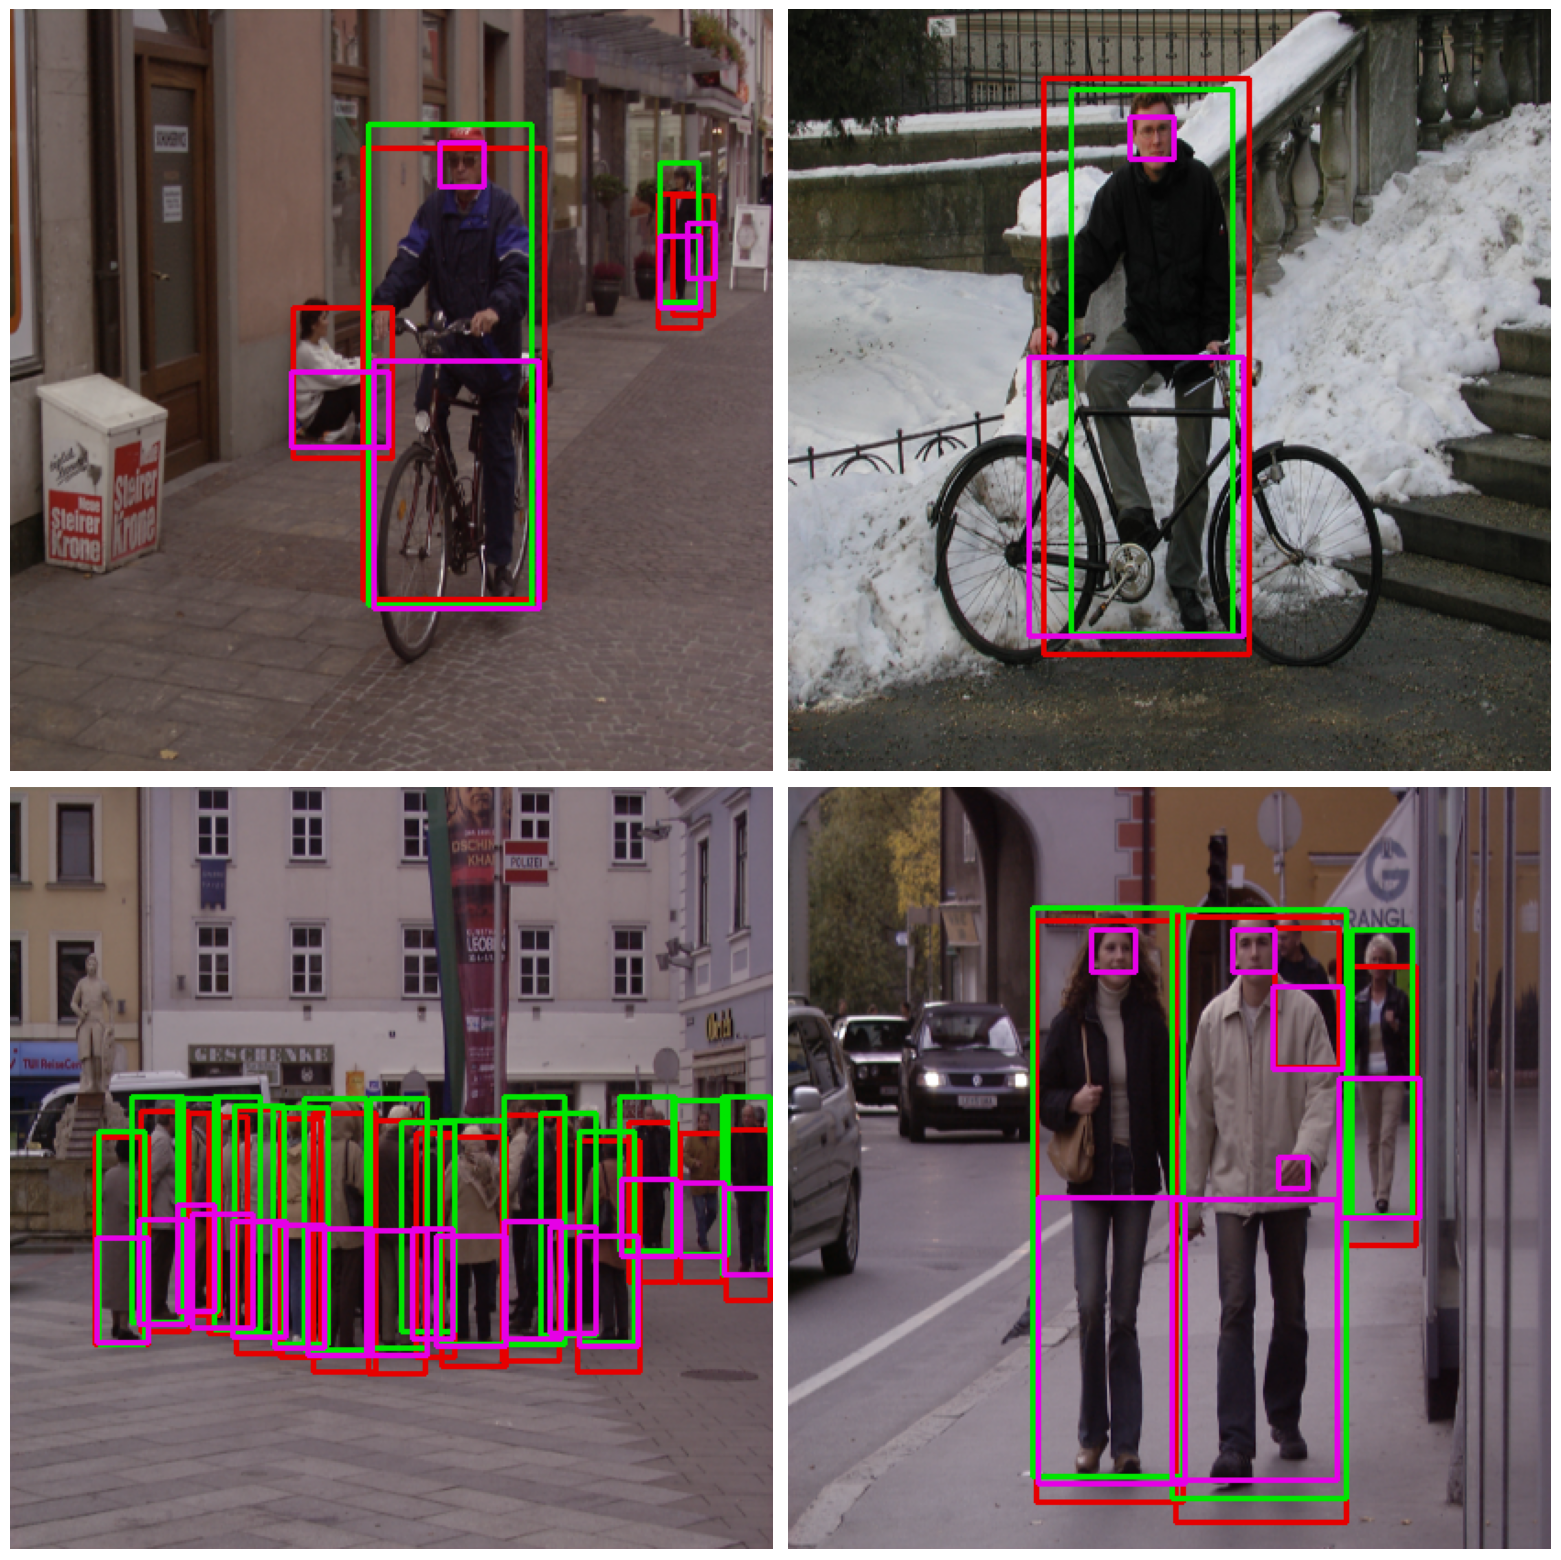
\includegraphics[width=1\textwidth]{other/figures/INRIA_samples_v2.png}
        \caption{INRIA Person}
    \end{subfigure}
    \begin{subfigure}{0.38\textwidth}
        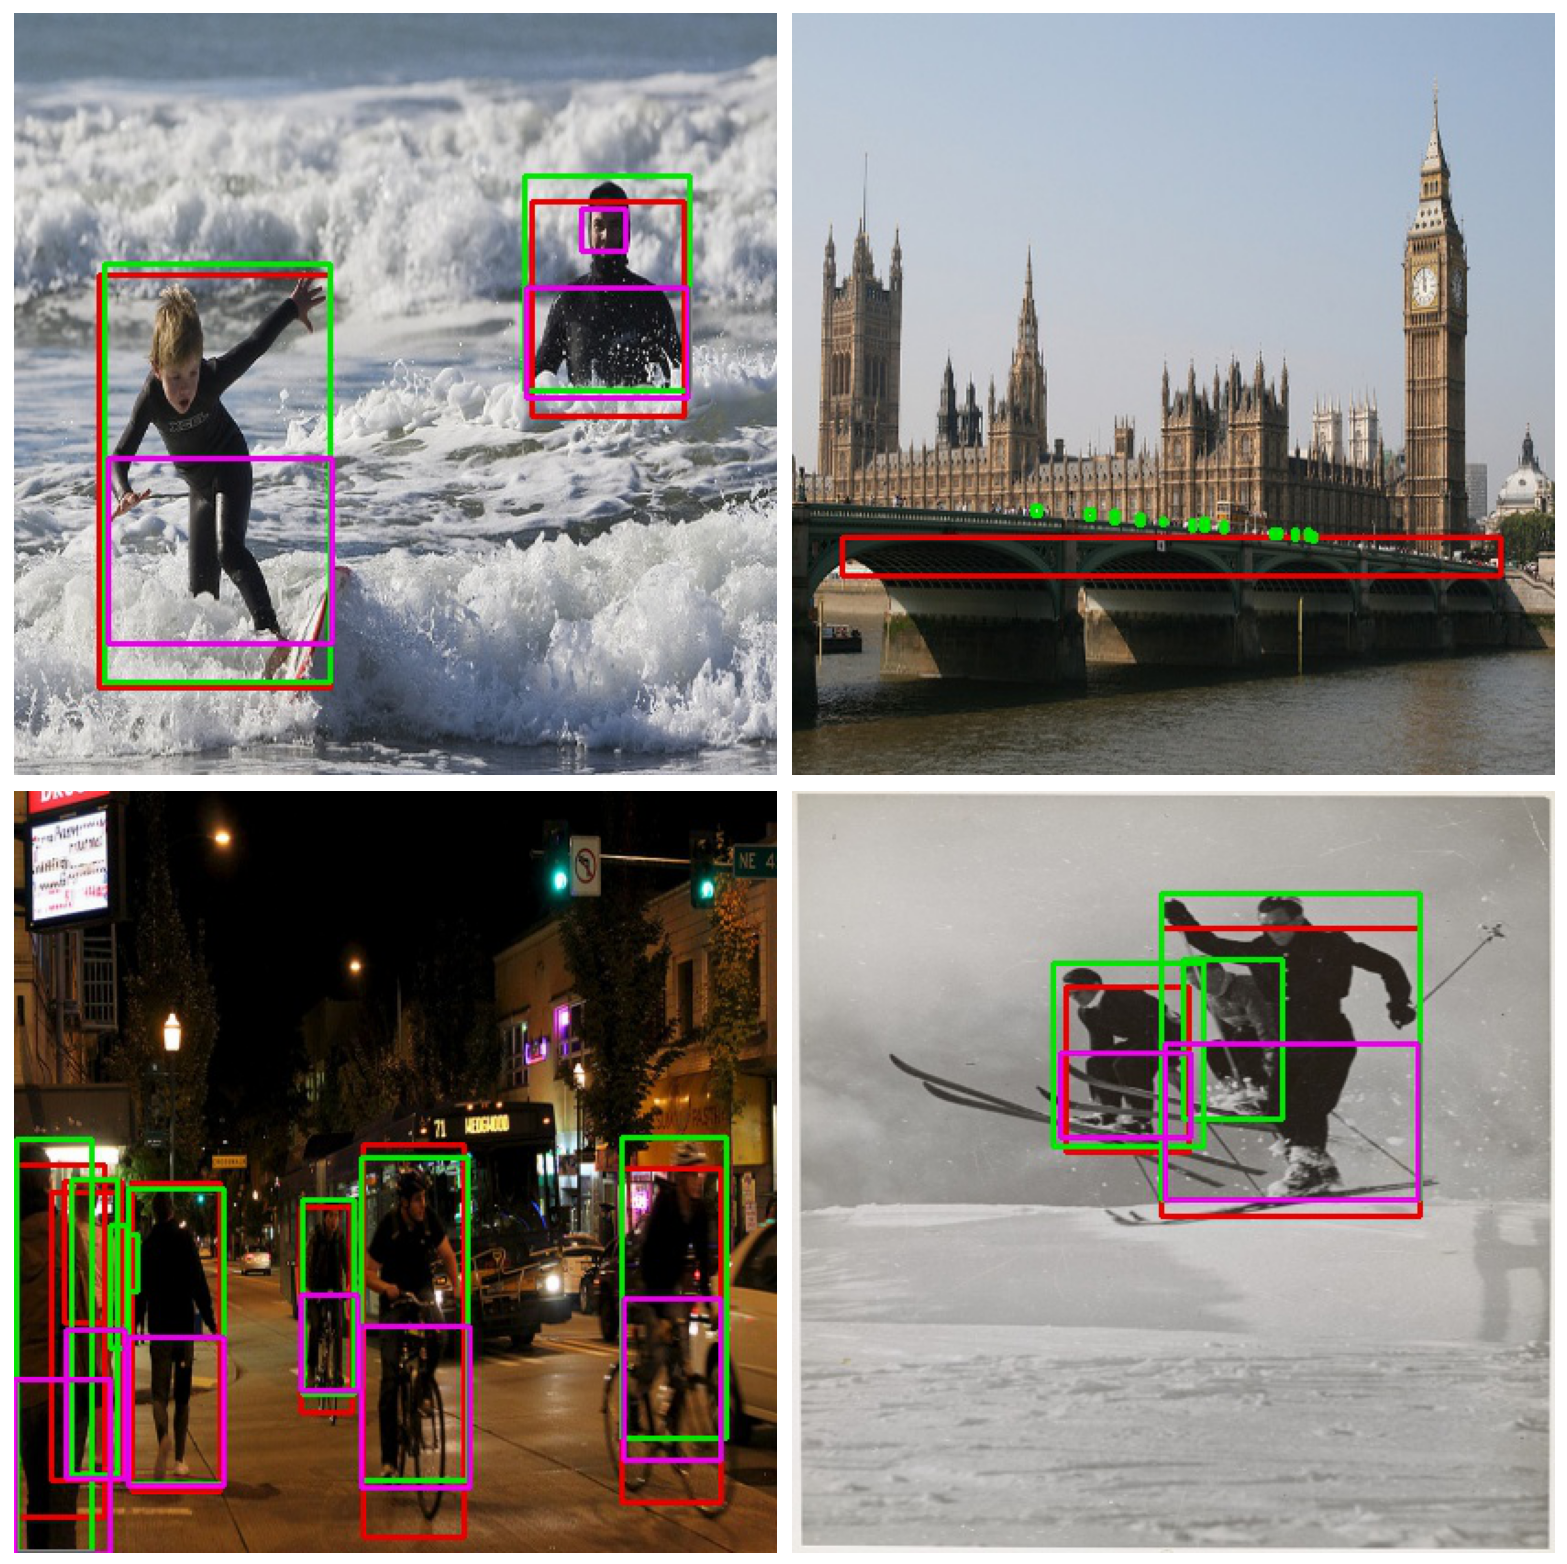
\includegraphics[width=1\textwidth]{other/figures/COCO_samples_v2.png}
        \caption{COCO}
    \end{subfigure}
    \caption{Images taken from INRIA Person and COCO datasets highlighting the main classifier predictions (red boxes), ground truth annotations (green boxes) and detected features specifications (magenta boxes) in the images.}
    \label{summary_pics}
\end{figure*}


\begin{figure*}[h]
    \centering
    \begin{subfigure}{0.4\textwidth}
        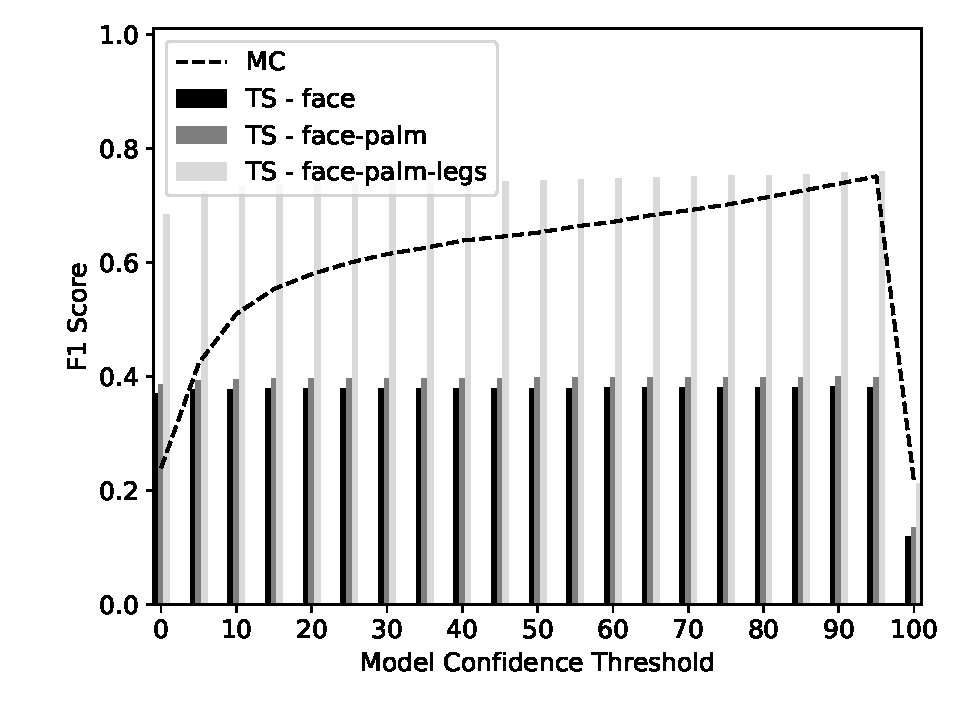
\includegraphics[width=1\textwidth]{other/figures/INRIA_exp_20_varying_features_.pdf}
        \caption{INRIA Person}
    \end{subfigure}
    \begin{subfigure}{0.4\textwidth}
        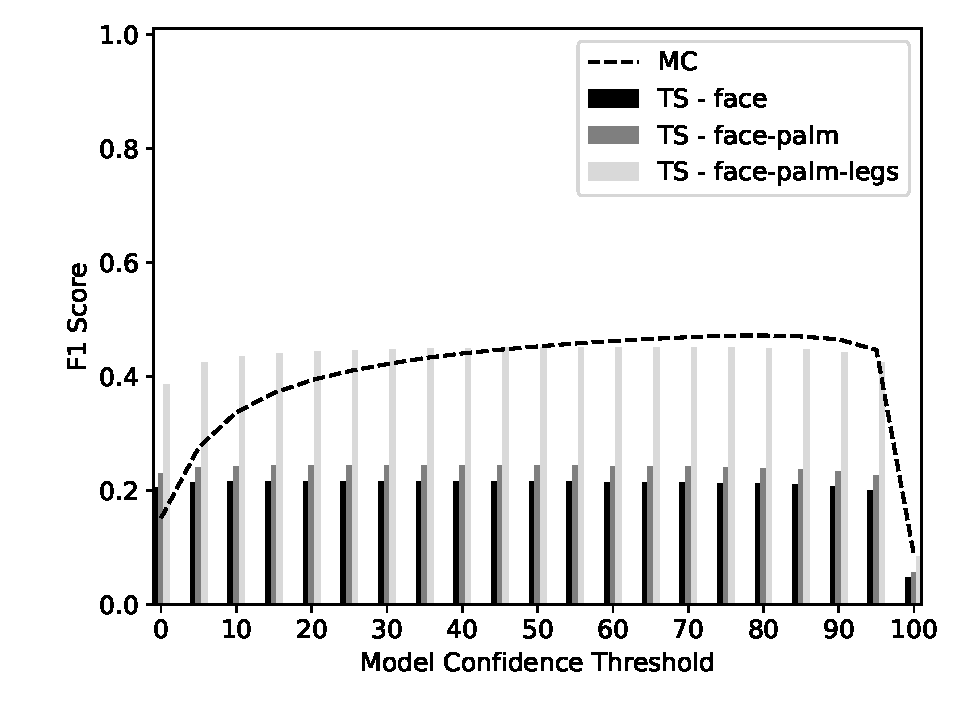
\includegraphics[width=1\textwidth]{other/figures/COCO_exp_19_varying_features_.pdf}
        \caption{COCO}
    \end{subfigure}

    \begin{subfigure}{0.4\textwidth}
        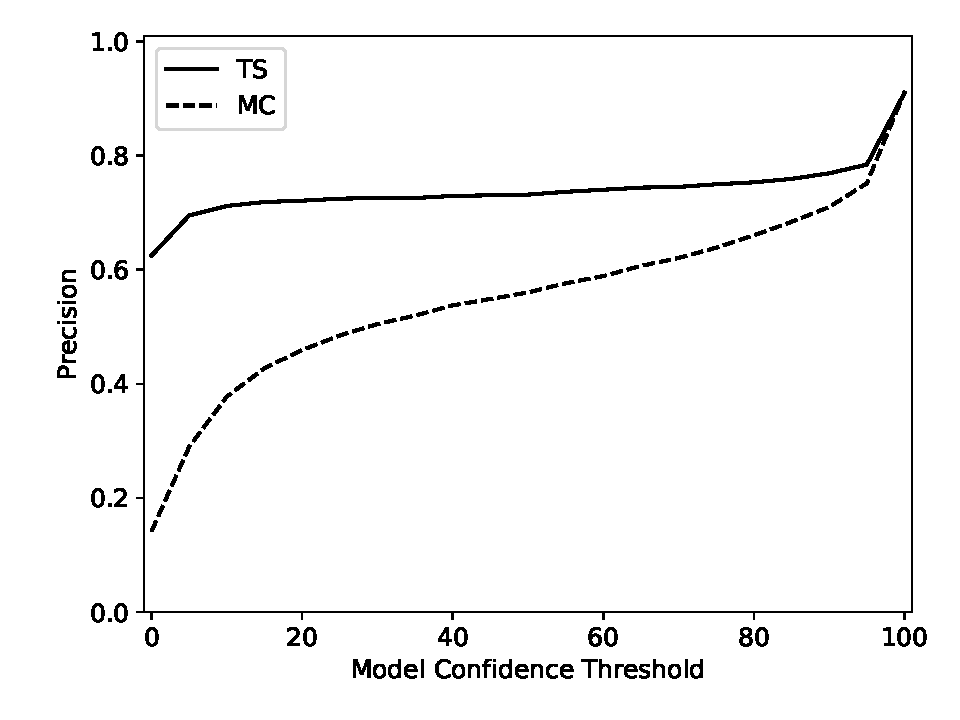
\includegraphics[width=1\textwidth]{other/figures/INRIA_exp_20_Precision.pdf}
        \caption{INRIA Person}
    \end{subfigure}
    \begin{subfigure}{0.4\textwidth}
        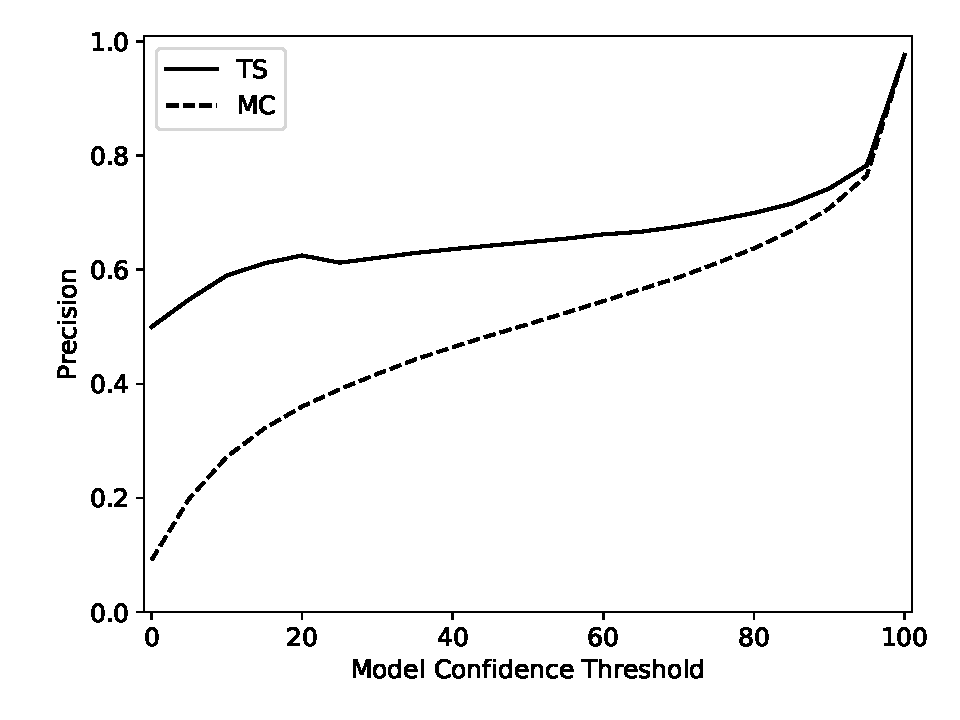
\includegraphics[width=1\textwidth]{other/figures/COCO_exp_19_Precision.pdf}
        \caption{COCO}
    \end{subfigure}
    \caption{Detect Trustworthiness}
    
    % \caption{Shows F1 score evaluation for the main classifier performed on the INRIA and COCO datasets. The dotted line shows the F1 score when relying on the model confidence alone to approve of trustworthy predictions. The bars represent the F1 score when relying on the TS to approve of predictions made by the main classifier for the different features specifications added incrementally. The results are shown across different model confidence thresholds of the main classifier.}
    \label{detect_trustworthiness}
\end{figure*}

\begin{figure*}[h]
    \centering
    \begin{subfigure}{0.4\textwidth}
        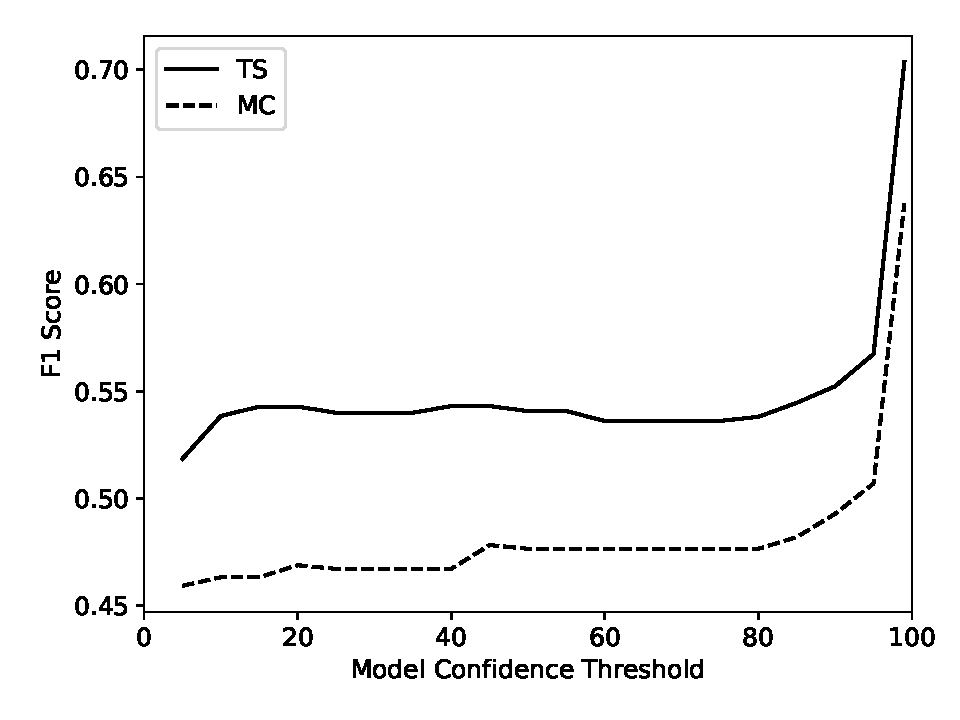
\includegraphics[width=1\textwidth]{other/figures/INRIA_exp_20_F1Score_SUS_VS_MC_untrustworthy_predictions.pdf}
        \caption{INRIA Person}
    \end{subfigure}
    \begin{subfigure}{0.4\textwidth}
        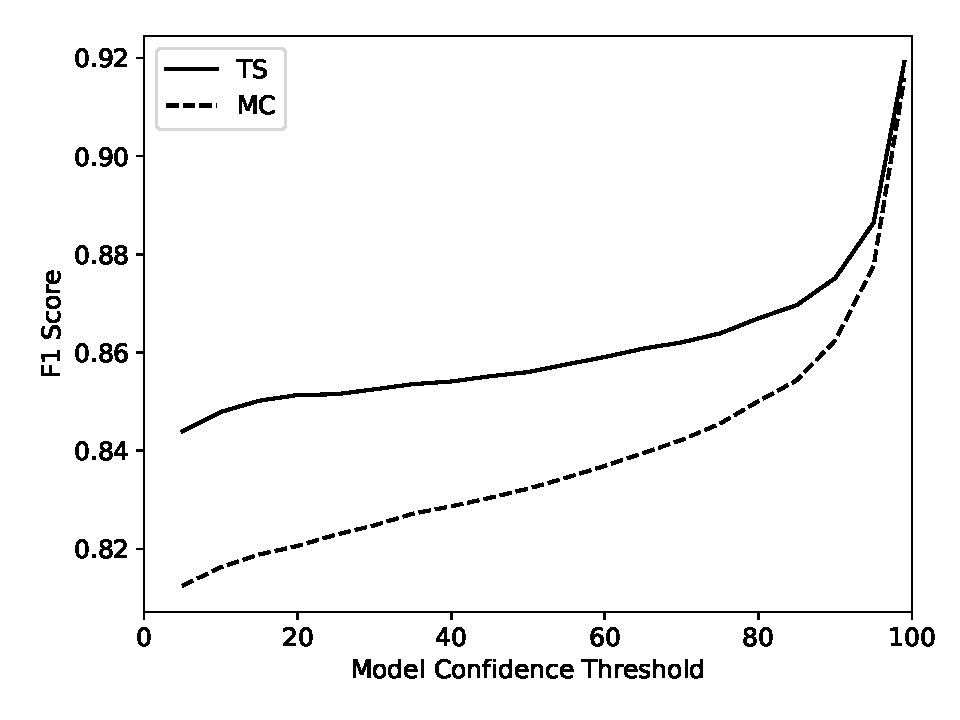
\includegraphics[width=1\textwidth]{other/figures/COCO_exp_19_F1Score_SUS_VS_MC_untrustworthy_predictions.pdf}
        \caption{COCO}
    \end{subfigure}

    \begin{subfigure}{0.4\textwidth}
        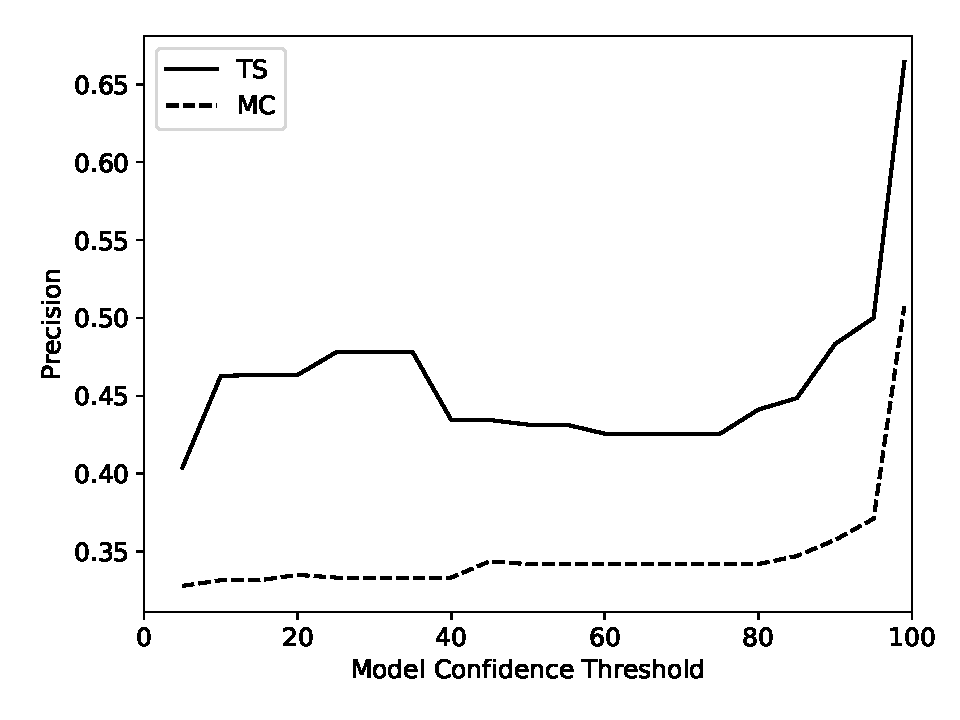
\includegraphics[width=1\textwidth]{other/figures/INRIA_exp_20_Precision_SUS_VS_MC_untrustworthy_predictions.pdf}
        \caption{INRIA Person}
    \end{subfigure}
    \begin{subfigure}{0.4\textwidth}
        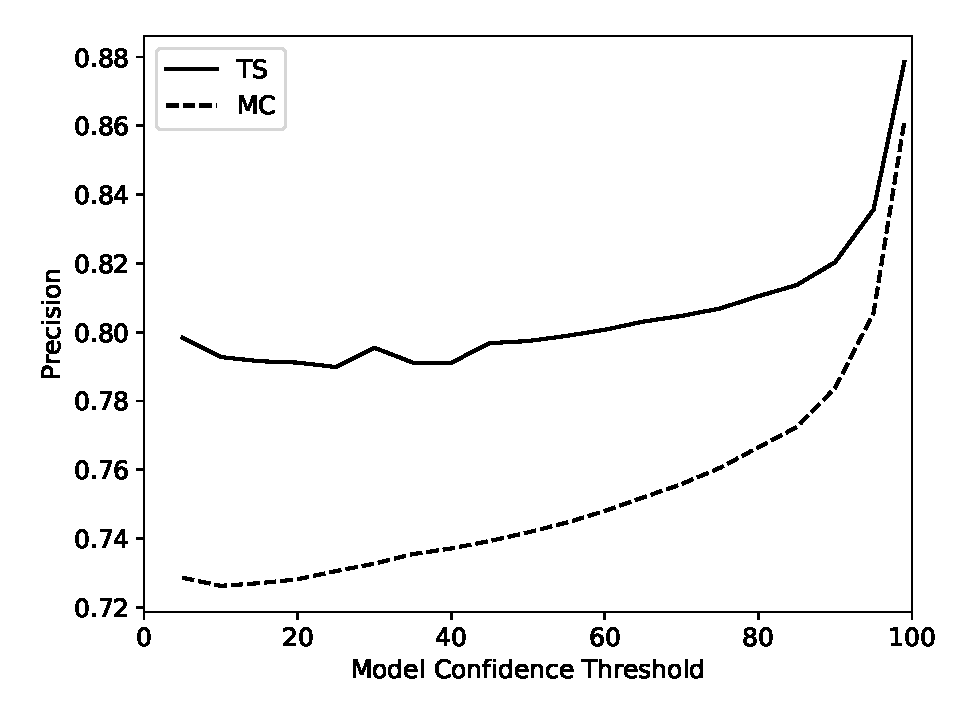
\includegraphics[width=1\textwidth]{other/figures/COCO_exp_19_Precision_SUS_VS_MC_untrustworthy_predictions.pdf}
        \caption{COCO}
    \end{subfigure}
    
    \caption{Detect Suspiciousness}
    \label{detect_suspiciousness}
\end{figure*}

\section{Experimentation Setup} \label{sec:experiment}
We used the application of person detection using CNNs to advocate our method in both identifying trustworthy predictions and detecting suspicious frames. 
% Suspicious frames in this context is used to refer to frames or images with false negatives.
%
The effectiveness of trustworthiness detection in predictions using the trustworthiness score (TS) method is evaluated against model confidence (MC) as our baseline. 
%
The baseline for assessing the effectiveness of the suspiciousness score in detecting suspicious frames is also based on MC.
%
In this case the baseline considers a frame to be suspicious if the main classifier outputs predictions with model confidence below the model confidence threshold. 
%
In the rest of this section we discuss further details for our experimentation setup.

% in prediction is evaluated against the model confidence (MC) in prediciton as the baseline.
%
% to develop examples of features specifications and their usage in calculating the trustworthiness score. 
%
% We compare the trustworthiness score evaluation against ground truth annotations to evaluate the method's effectiveness at assessing the main classifier's performance.
% We compare the trustworthiness score evaluation against ground truth annotations to evaluate the method's effectiveness at assessing the main classifier's performance.

\subsubsection{Main Classifier}
For any given application, the \textit{main classifier} is the CNN responsible for detecting the object of interest, in this case study the object of interest is a person. 
%
A YOLO~\cite{Redmon2015} object detector pre-trained on the COCO dataset~\cite{COCO_dataset} was chosen to act as the main classifier in our case study. The choice of using YOLO as the main classifier was based on its growing utilisation and popularity in the machine learning community. In addition, to the simplicity provided in its integration via PyTorch and the documentation availability through GitHub~\cite{Jocher_YOLOv5_by_Ultralytics_2020}. 
%
The YOLO object detector outputs a label, bounding box and model confidence for the detected objects. The bounding box can conveniently serve as the explanation to the prediction, whilst the model confidence provides the baseline to evaluate the effectiveness of the trustworthiness score.

\subsubsection{Features specifications}
In the task of detecting a person we identify (using human logic) three main distinctive features. We list them as features specifications below\footnote{The method used in writing down the specifications is based on NASA guidelines for writing requirements and specifications.~\cite{NASA_SystemsEngineeringHandbook}.}:
\begin{itemize}
    \item  A person detection in an image shall include the facial landmarks of a human.
    \item A person detection in an image shall include a human palm.
    \item A person detection in an image shall include the legs of a human.
\end{itemize}

For all three listed features specifications we used object detectors to describe the features in machine interpretable form for monitoring. 
%
As observed we only provided the specification-text part of a feature specification and eliminated the usage of a specification-visual. 
%
This is becuase we used existing pretrained object detectors as monitors for our features specifications, allowing us to overcome the need to build datasets for the specification-visual.
% to produce a specification visual from which one would usually construct the feature specification monitor.
%
% we used existing pretrained models and synthesized datasets. mainly on using pre so we avoided the need of building a dataset to express these features.  

Pre-trained models for detecting faces and hands were used to monitor for the first two specifications. 
%
For detecting faces a pre-trained model based on Dlib was used~\cite{king2015}.
For the detection of palms MediaPipe-Hands by google research was used~\cite{mediapipe}.
%
For the the third specification of legs detection, a pre-trained model for detecting legs was not found, therefore, we trained our own custom legs object detector using the YOLO5s~\cite{Jocher_YOLOv5_by_Ultralytics_2020} architecture on a synthesised legs dataset. The legs dataset was synthesised by taking the lower half of the person labels in the COCO dataset and labeling them as legs.
%
% Using the NASA shall statments format for specificaitions
% - Setup description:
%
% -- palm detection
% -- face detection
% -- Legs detection
%
\subsubsection{Datasets}
Two datasets were used in our evaluation: 1) INRIA Person dataset~\cite{Dalal2005} (dataset size: 902 images) and 2) COCO dataset~\cite{COCO_dataset} (dataset size: 328,000 images). 
%
The INRIA dataset has served as a lightweight dataset for development and early testing, whilst the COCO dataset is used to ensure the method scales.% to larger datasets.

% \subsubsection{Evaluation metrics} 
% We use Precision and F1 Score to evaluate our method.
% For Trustworthiness
% Precision  
% Recall
% F1 Score
% For suspicoiusness
% The model confidence 
% \todo[inline]{Conitnue here}

\subsubsection{Hyperparameters selection}
There are two hyperparameters associated with the trustworthiness score (TS): $\beta$ and TS threshold. For all experiments, we set $\beta = 1$ for all features specifications. The TS threshold (or the SS threshold in the case of detecting suspiciousness) is varied to maximise the F1-Score of the TS method approved predictions.


\section{Results and Discussion} \label{sec:results}
To evaluate our method we analyse against ground truth the counts of True Positives (TP), False Positives (FP) and False Negatives (FN) for trustworthy predictions based on 1) the model confidence only then 2) the trustworthiness score.  
%
The metrics often used to analyse TP, FP and FN are Precision, Recall and F1 score. Precision is calculated as $\frac{TP}{TP+FP}$  which is meant to convey how many of the predictions are accurate out of all predictions made. Recall on the other hand expresses the rate of the classifier getting correct predictions. This is calculated as $\frac{TP}{TP+FN}$. Often as one tries to increase Precision, Recall tends to decrease as a result. Ideally one aims to maximise both Precision and Recall. The F1 score is used to express the maximisation of both precision and recall simultaneously. This is given by $\frac{2\cdot Precision\cdot Recall}{Precision + Recall}$.
%
The aim of our approach is to improve the Precision whilst at least keeping the F1 Score (more or less) the same or improving it. 
%
Therefore, in our results we mainly focus on Precision improvement but we also plot the F1 score for completeness. 
%

% \todo[inline]{change x- axis to be Accuracy of main classifier.}
%
\subsubsection{Features specifications sufficiency}
Under representation of objects using features specifications can naturally lead to the F1 Score based on TS to be less than on MC. Therefore, the first criterion we assess is the sufficiency of features used to represent the object being classified.
%
Figure~\ref{detect_trustworthiness} (a) to (b) shows the F1 score of the main classifier for the INRIA dataset and the COCO dataset. The F1 score when relying on the model confidence alone to approve of trustworthy predictions is shown by the dotted line. The bars represent the F1 score when relying on the TS to approve of predictions made by the main classifier. The bars are shown for three TS setups, in each setup a feature specification is added incrementally. 
%
The results are shown for different accuracies of the main classifier. 
%
As can be seen for both datasets in Figure~\ref{detect_trustworthiness}, the F1 score for our TS method gives poorer performance than the MC when using only the face as a feature specification, with a slight increase when adding the hand feature specification, and then surpasses the MC performance when adding in the legs feature specification. 
%
This shows how sufficient representation of an object using feature specifications is crucial for the effectiveness of our approach.

% based on the first two specifications gives poorer performance than if relied on the  the F1 score 

% tends to be significantly lower than the MC when using only the face as a features specification, with a slight increase when adding the hand features specification and shooting to an F1 score of 0.9 with adding in legs, making the TCS approach very close in to the GT line.
 

\subsubsection{Detect Trustworthiness}
Figure~\ref{detect_trustworthiness} (c) to (d), shows how the performance based on precision changes with the accuracy of the main classifier for both the INRIA and the COCO datasets. It can be noticed that the trustworthiness score consistently performs better than the model confidence alone, with the amount of improvement decreasing as the accuracy of the main classifier increases. 
%
It can be observed using Figures ~\ref{detect_trustworthiness} (a) to (d), that the trustworthiness score approach significantly improves the precision, whilst also improving or maintaining the F1 score to a level equivalent to that provided by the model confidence alone.  
%
Observing the precision plots in Figure ~\ref{detect_trustworthiness} our method provides an improvement of approximately 40\% for low model confidence thresholds and diminishes to zero for high model confidence thresholds, averaging to approximately 20\% improvement when averaged across different model confidence thresholds.


% We use \textit{model confidence threshold} to refer to the min accuracy required in a prediction made by the main classifier above which predictions are .


\subsubsection{Detect Suspiciousness} 
Similar to results shown for detect trustworthiness, Figure~\ref{detect_suspiciousness} (a) to (d) show cases the effectiveness of the TS metric if modified to the suspiciousness score to calculate the suspiciousness in a frame. 
%This is compared against the model confidence as our baseline. 
As can be seen the TS approach provides a significant improvement compared to relying on MC only. Similar to our observation in detect trustworthiness, this effectiveness diminishes as the model confidence threshold of main classifier increases.
%
Examining the precision plots in Figure ~\ref{detect_suspiciousness} our method provides an improvement of approximately 10\% for low model confidence thresholds and diminishes to zero for high model confidence thresholds, averaging to approximately 5\% improvement when averaged across different model confidence thresholds.


% \todo[inline]{Check I do describe the baseline for trsutworhtiness and Add baseline for suspicoiusneess: The baseline used here again relies on the model confidence. For a frame to be suspicious based on model confidence means that the main classifier outputted predictions below the selected main classifier's accuracy. }


% shows how the performance based on precision 
% changes with the accuracy of the main classifier for both the INRIA and the COCO datasets. It can be noticed that the trustworthiness score consistently performs better than the model confidence alone, with the amount of improvement decreasing as the accuracy of the main classifier increases. 
% %
% It can be observed using Figures ~\ref{detect_trustworthiness} (a) to (d), that the trustworthiness score approach significantly improves the precision, whilst also improving or maintaining the F1 score to a level equivalent to that provided by the model confidence alone.  



\subsubsection{Limitations}
Whilst the TS presents a promising approach for improving detection of trustworthy predictions and suspicions frames during operation, the method may still suffer from out of distribution classification issues, especially that features specifications detection relies on other CNNs.
Therefore, methods for detection of out of distribution environments (e.g. dissimilarity measures~\cite{Hond2020}).) are very complimentary to our method.
% from the classic issue that classifiers face. That is to fail detecting features specifications in an image due to the input data falling out of the training data distribution. 
% Therefore, the TCS approach should be complimented with monitoring for dissimilarity of inputted data with the training distribution (e.g. dissimilarity measures~\cite{Hond2020}). 
% \todo[inline]{Note to add: our method may be limited to asisting with detecting in-distribution erroneous predictions, but may questionable for out-of-distribution samples where the features specifications themselves may fail to be detected. Therefore, other works on dissimilarity measures, which focuses more on detecting out of distribution samples is a  complimentary field of work to our paper.}

% \todo[inline]{Add discussion on AMLAS to emphasis on the need for defining the operation environment \cite{hawkins2021guidance}}
% The distance of objects predicted should be taken into account when counting TP, FP, FN for both GT and TCS this may affect the evaluation of the TCS approach significantly. Objects that are are very small or far in an image would be significantly more difficult to analyse and detect features specifications in it. In fact the definition of object distances for prediction ideally should form part of the specifications for the whole system as is demonstrated in some publications e.g.\cite{Gauerhof2020}. 

% Furthermore, we list some applications for our method below: 
% \begin{itemize}

%     \item The method presented in this paper can also serve as a powerful tool for automated post accident investigation analysis to determine the cause of an accident if was caused by a classifier's miss-detection. This very much compliments other tools for post accident investigations, such as an ethical black box~\cite{Winfield2017}.  

%     \item Help developers analyse and capture new data that may merit the classifier's training.

%     \item Speed up the labeling process of new data by initiating approximated labels based on features specification detection that can be altered by the ground truth (a human) to create accurate labels for new data more efficiently.

% \end{itemize}


\section{Conclusions} \label{sec:conclusions} 
We have introduced a method for quantifying and calculating trustworthiness score (TS) in a classifier's predictions by monitoring for features specifications.
%
We found that the number and type of monitored features specifications used in calculating TS is critical to the effectiveness of the approach.
%
We have also explored if a modification of TS can be used to help with the detection of suspicious frames (i.e. frames containing false negatives) via calculating a suspiciousness score. 
%
Overall, our method showed an improvement compared to using model confidence of a classifier in detecting trustworthy predictions and suspicious frames. 
%
Our method provides an averaged improvement of 20\% and 5\% for detecting trustworthiness and suspiciousness respectively. 

% in classification score (TCS), by monitoring for features specifications in an image. Effectively producing a form of an automated ground truth (GT).
%
% We found that the number and type of monitored features specifications used in calculating the TCS is crucial to the effectiveness of the approach in representing the GT during operation. 
% 
% Furthermore, to sufficiently evaluate the reliability of the TCS approach in representing the GT, one needs 1) a complete ground truth (no missing annotations); 2) a definitive set of specifications followed in both labelling of the ground truth and in training the features monitors used in calculating the TCS. 
%
% The latter will also allow for one to maximise the effectiveness of the TCS in representing the GT. 
%
% Not much focus has been devoted in maximising the reliability of TCS in representing the GT in our case study as this is beyond the scope of this paper but this remains as a future goal for this work.


\section*{Acknowledgments}
This research is part of an iCASE PhD funded by EPSRC and Thales UK. 
Kerstin Eder was supported in part by the UKRI Trustworthy Autonomous Systems Node (grant number EP/V026518/1).
%
Thanks to Edwin Simpson from University of Bristol and Darryl Hond from Thales for helping with reviewing.
